\section{Konzeption und Umsetzung}
\label{sec:4}
\subsection{Idee}

Da die Ergebnisse dieser Arbeit relevant für das KoViTReK Forschungsprojekt\footnote{\url{https://www.th-koeln.de/anlagen-energie-und-maschinensysteme/kovitrek\_87259.php}}
sein könnten und dieses in der Laufzeit- und Entwicklungsumgebung Unity\footnote{\url{https://unity.com}}
implementiert werden soll, werden auch die Partikelsysteme in der selben Umgebung entworfen.
Der erste Ansatz basiert auf aufwändig vorberechneten Simulationen, welche in einem Texture Sheet gespeichert werden und daraufhin den Einsatz in Unity
sehr effizient und realistisch machen. 


\subsection{Erstellung der Texturen}
\label{sec:4.1}
% \subsubsection{Texture Sheets}


Die Texturen werden auf zwei verschiedene Arten erstellt. Für die Variante mit Parallax Occlusion Mapping werden zwei
Texturen in der von SideFX entwickelten 3D-VFX-Grafiksoftware Houdini \footnote{\url{https://www.sidefx.com/products/houdini/}} erstellt. 
Houdini bietet die Möglichkeit relativ einfach und schnell physikalisch basierte und visuell überzeugende Rauch- und Feuersimulationen zu erstellen. 
Die Simulationen basieren auf Fluidberechnungen, wodurch ein realistisches Verhalten erzeugt und durch eine Vielzahl an Parametern beeinflusst werden kann.
Eine Möglichkeit die Houdini bietet, ist das Rendering der Animation in verschiedene Layers. So kann jedes einzelne Licht separat berechnet, gerendert und 
hinterher vorallem verwendet werden. Dazu werden Lichtquellen wie in \autoref{fig:lightSetup} aus allen sechs Richungen zum Rauch hin angeordnet, 
sodass jeweils eine Seite beleuchtet wird. Die Animation des Rauchs wird daraufhin in eine sich selbst loopende Animation geschnitten und als einzelne Frames gerendert.

\begin{figure}[h!]
    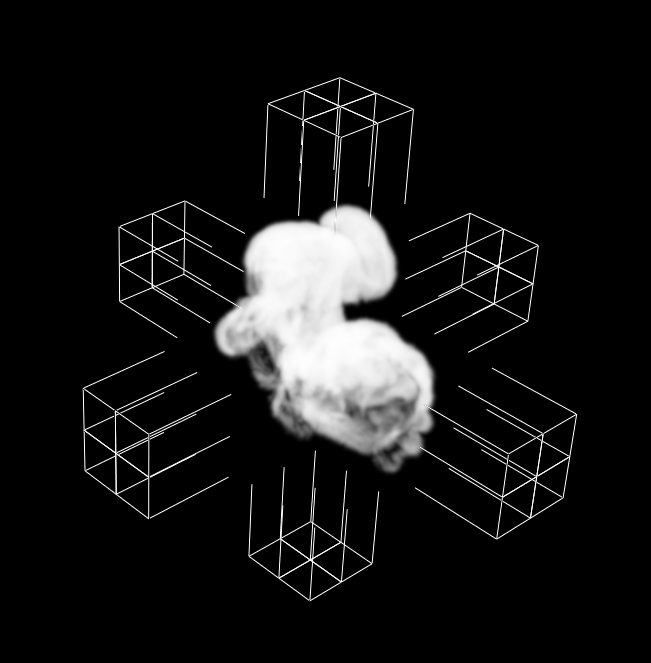
\includegraphics[width=0.49\textwidth]{Grafiken/Implementation/Lightmaps/Smoke_LightSetup.png}
	\centering
    \begin{footnotesize}
        \caption{Schritte um Loop einer Rauchanimation ohne sichtbaren Schnittzu erzeugen. }
		\label{fig:lightSetup}
    \end{footnotesize}
\end{figure}


% Die Animation wird daraufhin in einzelnen Frames auf einer Textur in einem Grid abgespeichert, auch Texture Sheet, Sprite Sheet oder Flipbook genannt.
% Jeder Frame wird in der Textur mit einer Auflösung von 128 x 128 px gespeichert. Bei einer Frameanzahl von 8x8 = 64 Frames entspricht das also
% einer Auflösung der ganzen Textur von 1024 x 1024 px.
% In jedem Frame werden in Textur 1 die Tangent-Lightmaps (Top/Left/Right) in den jeweiligen RGB-Channels gespeichert.
% Der Alpha-Channel enthält die Bottom-Lightmap. In Textur 2 wird eine Heat-/Emissionmap im Rot-Channel gespeichert, die Alphainformation im
% Grün-Channel und die für das Parallax-Occlusion-Mapping benötigte Heightmap im blauen Farbkanal. Der Alpha-Channel wird hierbei nicht benutzt und könnte frei mit weiteren 
% Informationen gefüllt werden. 
%Diese Art Informationen in die Texturkanäle zu speichern ersetzt

\begin{figure}[h!]
    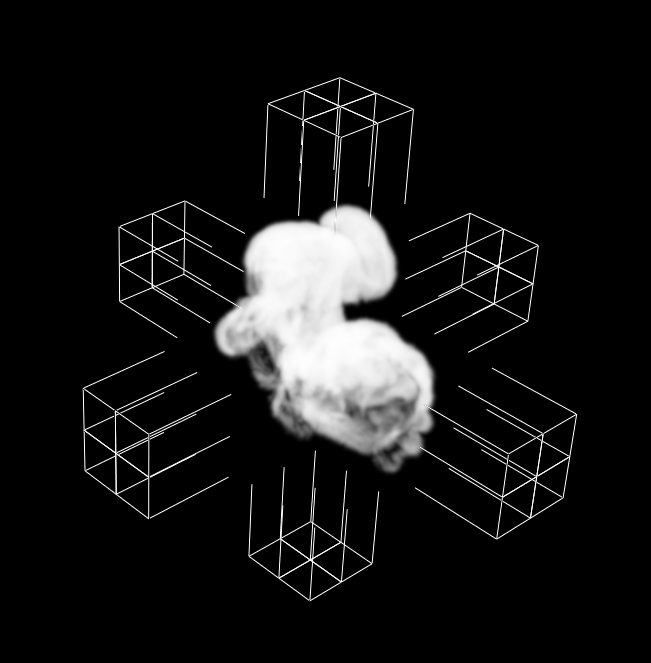
\includegraphics[width=0.49\textwidth]{Grafiken/Implementation/Lightmaps/Smoke_LightSetup.png}
	\centering
    \begin{footnotesize}
        \caption{Setup der Beleuchtung der Rauchsimulation in Houdini.}
		\label{fig:lightSetup}
    \end{footnotesize}
\end{figure}


\begin{figure}[h!]
	\centering
		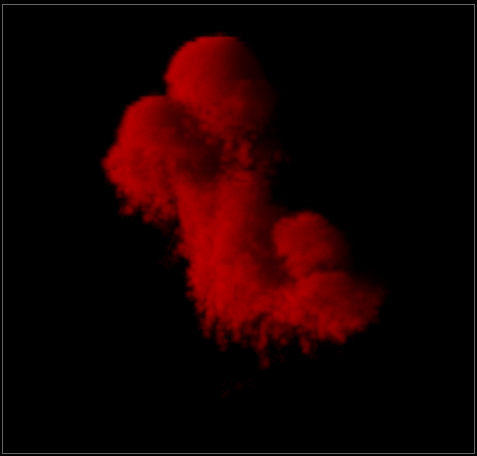
\includegraphics[width=0.24\textwidth]{Grafiken/Implementation/Lightmaps/T1_R.png}
		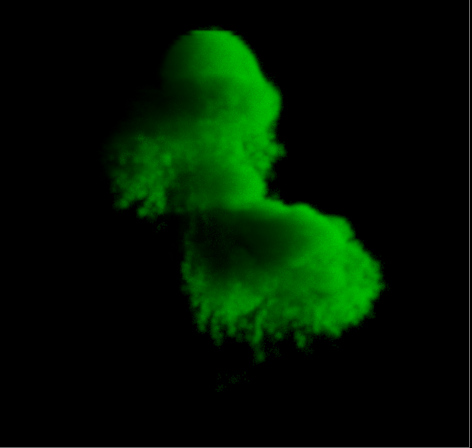
\includegraphics[width=0.24\textwidth]{Grafiken/Implementation/Lightmaps/T1_G.png}
		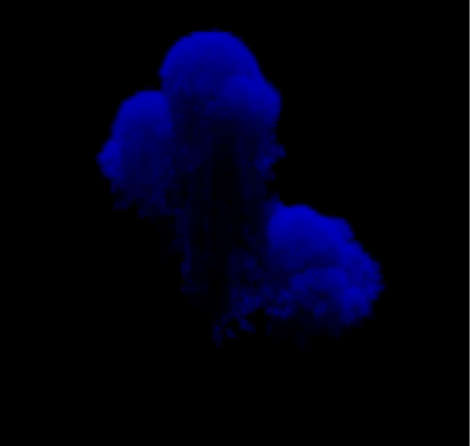
\includegraphics[width=0.24\textwidth]{Grafiken/Implementation/Lightmaps/T1_B.png}
		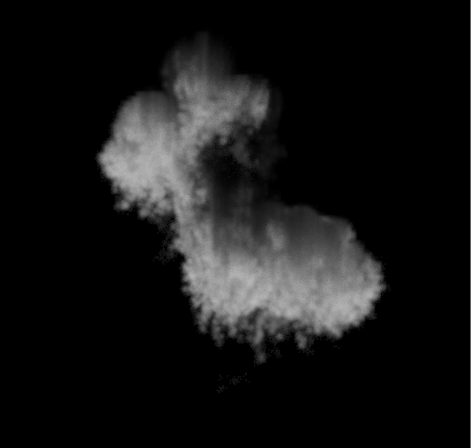
\includegraphics[width=0.24\textwidth]{Grafiken/Implementation/Lightmaps/T1_A.png}
	
    \begin{footnotesize}
        \caption{Setup der Rauchsimulation in Houdini. Links ist beispielhaft ein Frame der Simulation in seine Farbkanäle aufgeteilt. 
        Die Richtungen aus denen der Rauch jeweils beleuchtet wurde ist dabei gut zu erkennen. }
    \end{footnotesize}
	\label{fig:lightDirections}
\end{figure}


\begin{figure}[h]
	\centering
	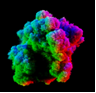
\includegraphics[width=0.49\textwidth]{Grafiken/Implementation/T1_RGB.png}
	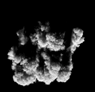
\includegraphics[width=0.49\textwidth]{Grafiken/Implementation/T1_A.png}
	\begin{footnotesize}
		\caption{links: T1(RGB), rechts: T1(A)}
	\end{footnotesize}
	\label{fig:combinedChannel}
\end{figure}

\begin{figure}[h!]
	\centering
	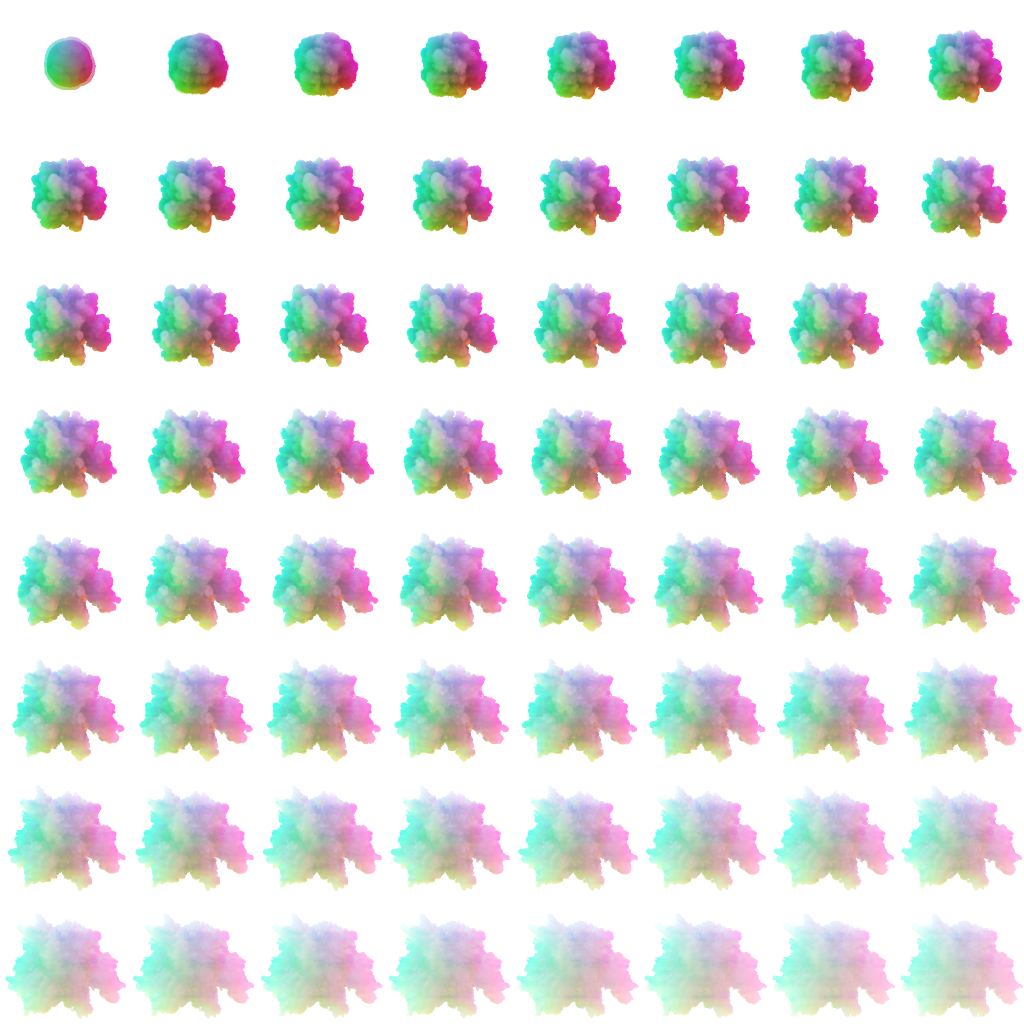
\includegraphics[width=0.49\textwidth]{Grafiken/Implementation/Explo_T1_8x8.png}
	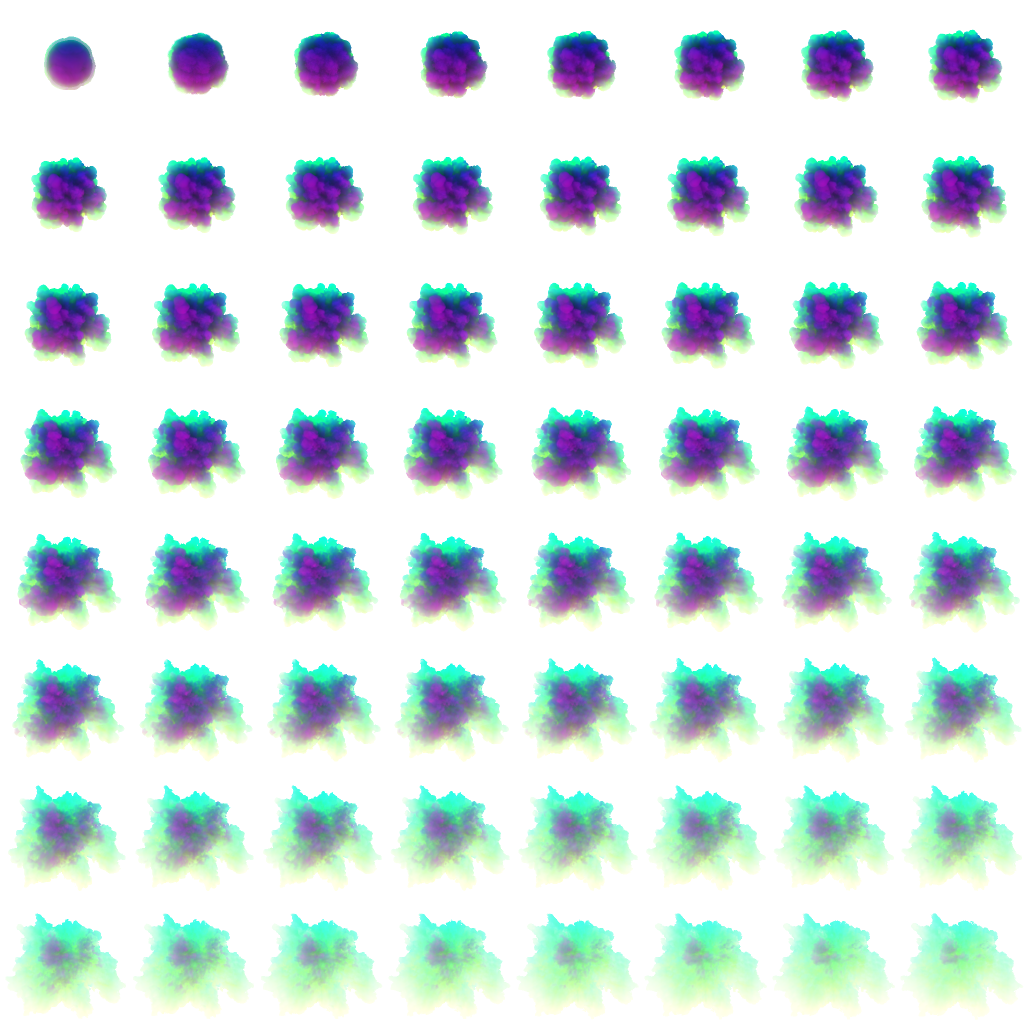
\includegraphics[width=0.49\textwidth]{Grafiken/Implementation/Explo_T2_8x8.png}
	\begin{footnotesize}
		\caption{Exportierte Spritesheets aus der Rauchsimulation in Houdini. Beide Bilder zeigen die selbe Simulation mit unterschiedlichen Beleuchtungsrichtung des Rauchs aus 
        den jeweiligen Richtungen. Links: Beleuchtung von rechts (R), links (G), oben (B) und den Alphawerten (A). 
        Rechts: Rauchsimulation beleuchtet von vorne (R), hinten (G), unten (B). Hierbei ist der Alphachannel noch frei.}
	\end{footnotesize}
	\label{fig:flipbook}
\end{figure}
\textcolor{red}{BILDER VON BEIDEN SPRITES}



In den beiden Texturen fehlen nun noch die Beleuchtung aus den Richtungen von Vorne und von Hinten. Diese werden allerdings im Shader
berechnet, anstatt sie in die Textur zu backen. Aus den verschiedenen Lightmaps kann daraufhin basierend auf der Richtung des Lichteinfalls
auf die Textur relativ günstig und performant eine korrekte Beleuchtung des Rauchs generiert werden.



\newpage
\textcolor{red}{\textbf{TODO:}} \newline
POM: \newline
- Alle Steps beschreiben\newline
- Grafiken einfügen\newline

RAYM: \newline
- Volumetextures generieren / downloaden\newline
- Vorgehen beschreiben\newline
- Grafiken \newline

% Raymarching: Volumetextures erstellen.
Diese werden mithilfe von prozedural generierten Noisetexturen erzeugt.
Daher basiert der zweite Ansatz auf dreidimensionalen Volumentexturen, welche mithilfe von Raymarching gesampled werden.


\subsection{Shader}
Für das Rendering der Partikel werden zwei Shader entwickelt. Diese basieren auf Parallax Occlusion Mapping und auf einem Raymarchingalgorithmus
durch eine Volumentextur. Für beide Algorithmen wird Unitys Shader Graph verwendet. Shader Graph ist, genau wie Unitys VFX Graph, ein Node-Editor um
schnell und übersichtlich Shader zu entwickeln. Hier besteht die Möglichkeit auch eigene Funktionen in Nodes zu verpacken und somit auf visuelle Art und Weise zu entwickeln.
Dies macht vorallem das Debugging einfacher und erlaubt das schnelle Prototyping von Ideen.
% Für den POM-Shader muss zuerst das Spritesheet 

Die Beleuchtung des Rauchs wird zuvor in Houdini durchsimuliert. Dabei wird nicht nur die Beleuchtung der Oberfläche aus verschiedenen Richtungen, 
sondern auch die Streuung, Reflexion und Absorption des Lichts innerhalb des Volumens berechnet und simuliert. 
Dies hat den Vorteil, dass diese aufwändigen Berechnungen des Lichts bereits gemacht wurden und in der Echtzeitanwendung lediglich zwischen verschiedenen 
Farbkanälen in der Textur interpolieren.


\subsubsection{Parallax Occlusion Mapping}


\subsubsection{Raymarcher}

Da Feuer und Rauch volumetrische Effekte ohne feste Oberfläche sind, lassen sich diese nicht wirklich durch Geometrie abbilden. Die Idee ist also ein
Volumen zu erzeugen und Strahlen durch dieses Volumen zu schicken, welches in festen Abständen das Volumen abtastet um daraus Informationen zu erhalten.
Hierbei wird das Licht, welches ebenfalls in dieses transluzente Volumen eindringt und absorbiert oder gebrochen wird, an jedem Samplepunkt berechnet.

Die Texturen werden daher wie in \textbf{\autoref{sec:4.1}} beschrieben durch generiertes Rauschen erzeugt.
% Um die notwendige Rechenleistung zu reduzieren, wird auch das generierte Rauschen in Texturen gebacken.  



\subsection{Partikelsystem}
Um die Partikelsysteme umzusetzen wird der relativ junge, von Unity entwickelte Editor 'Visual Effects Graph'
(kurz: VFX Graph) verwendet. VFX Graph ist ein nodesbasierter Editor, um schnell
dynamische und komplexe Partikelsysteme zu erzeugen\footnote{\url{https://unity.com/de/visual-effect-graph}}.
Im Gegensatz zum älteren Shuriken-Partikelsystem von Unity werden die Partikel hier auf der GPU
simuliert, wodurch das System deutlich an Performance gewinnt und ein mehr Partikel zeichnen kann.
Shuriken nimmt die Berechnungen im Gegensatz zum VFX Graph auf der CPU vor\footnote{\url{https://docs.unity3d.com/Manual/ChoosingYourParticleSystem.html}}.
Gerade für VR-Anwendungen bietet sich also dieses neue System an.
VFX-Graph hat jedoch nur sehr begrenzte Möglichkeiten, was Physiksimulationen und Kollisionen der Partikel angeht.
Es muss also ein System erstellt werden, welches trotz der Einschränkungen ein möglichst realistisches
Verhalten der Feuer- und Rauchpartikel gewährleistet.




\newpage
